\chapter{Интеграция норадреналиновой системы с серотониновой и дофаминовой системами.}
\label{chap:implementation}
Схема распространения норадреналина по мозгу была схематично изображена выпускником ИТИС 2016 года Д. Седленко. Эта схема представлена на рис. ~\ref{fig:nora_scheme}.


\begin{figure}
	\centering
	\includegraphics[width=\linewidth]{sedlenko}
	\caption{Схема распространения нейромедиатора норадреналин в мозге. Зелёными стрелками обозначен норадреналин, жёлтыми — глутамат, красными — ацетилхолин, синими — ГАМК, розовыми — дофамин. LC – голубоватое пятно, VTA - вентральная область покрышки, NTS – ядро одиночного пути, PGI - ядра paragigantocellular, PrH - perirhinal кора, LDT – латерально- спинное ядро покрышки, RN – ядра шва, BNST - слой ядра бороздки на терминале, Striatum – стриатум, Prefrontal cortex –префронтальная кора, Motor cortex –двигательная кора, Amy – миндалевидное тело, Thalamus – таламус, PVN –паравентикулярное ядро.}
	\label{fig:nora_scheme}
\end{figure}

Схема была реализована на языке python для инструмента моделирования нейронных спайковых сетей NEST-2.12.0. Каждой области мозга, указанной на схеме, было выделено биологически реалистичное для мозга крысы количество нейронов (данные о количестве нейронов собраны выпускницей ИТИС 2016 года Ю. Сафандеевой). Области мозга, в свою очередь, разбивались на подобласти, взаимодействующие с разными нейромедиаторами и друг с другом: например, ядрах шва есть два вида рецепторов норадреналина (на них выделено по 2900 нейронов) и серотониновые нейроны. Для активации источников норадреналина генераторы спайков должны быть подключены к зоне ядра одиночного пути, латерально-спинному ядру покрышки, вентральной области покрышки, перифинальной коре и паравентикулярному ядру.
Существуют аналогичные программные реализации систем дофамина (схема на рис. ~\ref{fig:dopa_scheme}) и серотонина (схема в общем доступе по ссылке https://github.com/research-team/NEUCOGAR/NEST). Различные области мозга, затрагиваемые нейромедиаторами на трёх схемах, были собраны в один словарь на python, количество нейронов на каждой – сохранено. Нейромодулирующие связи были последовательно подключены, и без добавления новых связей три схемы оказались соединены через вентральную область покрышки, префронтальную и моторную кору, ядра шва, миндалевидное и полосатое тело. Норадреналин, по схеме, должен возбуждать таламо - кортикальный цикл, в котором работает дофамин. Серотонин должен ингибировать центры дофамина, но возбуждать префронтальную кору, миндалевидное тело и гиппокамп. Норадреналин вызывает активность в ядрах шва, которые содержат центры серотонина, но последующее преодоление норадреналином ингибирующего влияния серотонина спорно. Ко всем частям мозга были подключены детекторы спайков и вольтметры.


\begin{figure}
	\centering
	\includegraphics[width=\linewidth]{dopa}
	\caption{Схема распространения нейромедиатора дофамин в мозге. Motor cortex – моторная кора, Striatum – полосатое тело, Gpe -- продольный бледный шар, Gpi – серединный бледный шар, STN – субталамическое ядро, Snc -- черная субстанция pars compacta, Snr – черная субстанция pars reticulata, Amygdala – миндалевидное тело, Thalamus – таламус.}
	\label{fig:dopa_scheme}
\end{figure}

При объединении трёх систем возникли следующие вопросы:


1) Будут ли работающие по предложенной модели нейромедиаторы вмешиваться в работу друг друга на уровне отдельных нейронов;


2) Как поведёт себя участок модели мозга при чрезмерной стимуляции.


3) Каким образом балансировать сильное ингибирующее влияние серотонина на систему с возбуждающим действием дофамина, который подвергается риску быть целиком подавленным;


4) Какой компьютер выдержит нагрузку в 500 000 нейронов с многочисленными связями, и как долго продлится одна подобная симуляция.


Для ответа на первый вопрос были проведены симуляции на простой сети из пяти нейронов: пресинаптический нейрон, постсинаптический нейрон, норадренергический нейрон, нейрон серотонина и нейрон норадреналина. К каждому нейрону были подключены детекторы спайков, вольтметры и генераторы спайков. Были проведены симуляции с включением одного из трёх нейромедиаторов при работающем другом нейромедиаторе, во всех комбинациях. Во всех случаях картина спайковой активности и динамики потенциала мембраны первого нейрона не изменялась, следовательно работа нейромедиаторов не саботирует друг друга на уровне отдельных нейромодулирующих нейронов. Пример показан на рис. ~\ref{fig:sero600voltage}: при включении на 600 миллисекунде серотонина, потенциал мембраны норадреналина продолжает находиться на уровне потенциала покоя, иногда происходит классический спайк. Концентрация норадреналина при этом подскакивает до максимума (рис. ~\ref{fig:sero600onNA}), поскольку событие «включение серотонина» для системы полностью неожиданное. На рис. ~\ref{fig:sero600onsynapse} показана динамика работы пресинаптического и постсинаптического нейронов, нейромодулировать которые призваны норадреналин и серотонин (происходит активное спайкование).

\begin{figure}
	\centering
	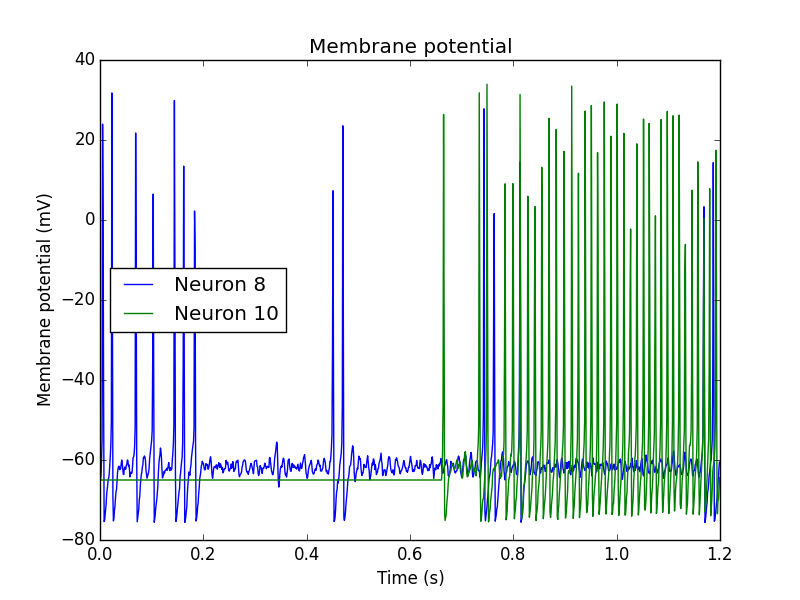
\includegraphics[width=0.5\linewidth]{sero600voltage}
	\caption{Изменение потенциала мембраны норадренергического нейрона (синий) и подключенного на 600 миллисекунде нейрона серотонина (зелёный).}
	\label{fig:sero600voltage}
\end{figure}

\begin{figure}
	\centering
	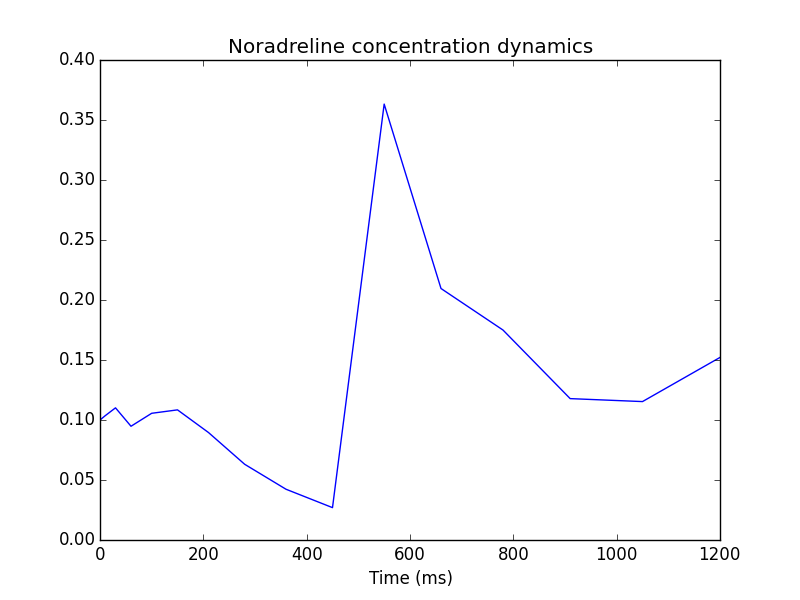
\includegraphics[width=0.5\linewidth]{sero600onNA}
	\caption{Изменение концентрации норадреналина при включении серотонина на 600 секунде.}
	\label{fig:sero600onNA}
\end{figure}

\begin{figure}
	\centering
	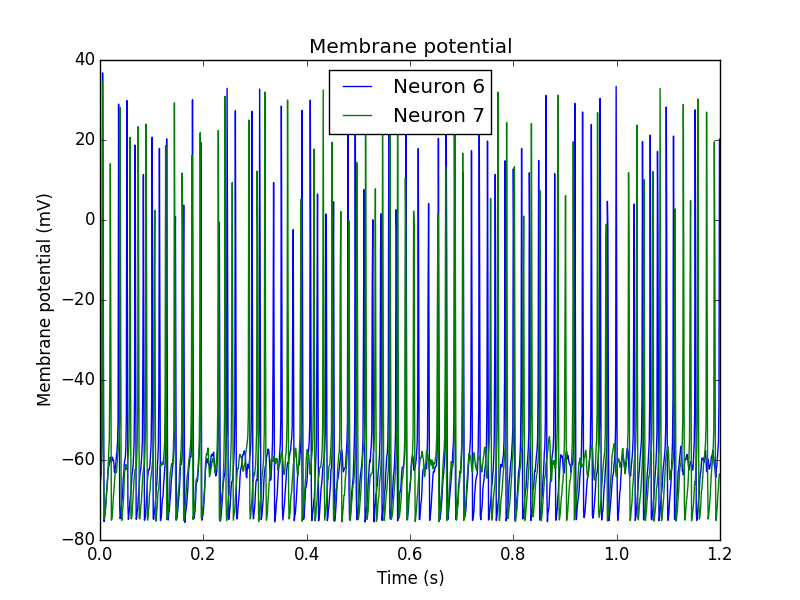
\includegraphics[width=0.5\linewidth]{sero600onsynapse}
	\caption{Изменение потенциала мембраны пресинаптического и постсинаптического нейронов при нейромодуляции.}
	\label{fig:sero600onsynapse}
\end{figure}

На вопрос о чрезмерной стимуляции отдельного участка мозга ядро NEST версии 12 дало неожиданный результат: пробный запуск модели в 1000 нейронов дал нереалистичное изменение потенциала нейронов в миндалевидном теле (рис. NN). Потенциал зацикливается вокруг -20 мВ, что не является потенциалом покоя и противоречит биологии, подобная ошибка стала возможна лишь из-за того, что в симуляции нейроны не сохраняют химические свойства, являются объектами с математическими характеристиками. Так как вопрос стоит на уровне версии NEST, то на данный момент он временно обойдён сокращением объёмов стимуляции у перестимулированных зон.


\begin{figure}
	\centering
	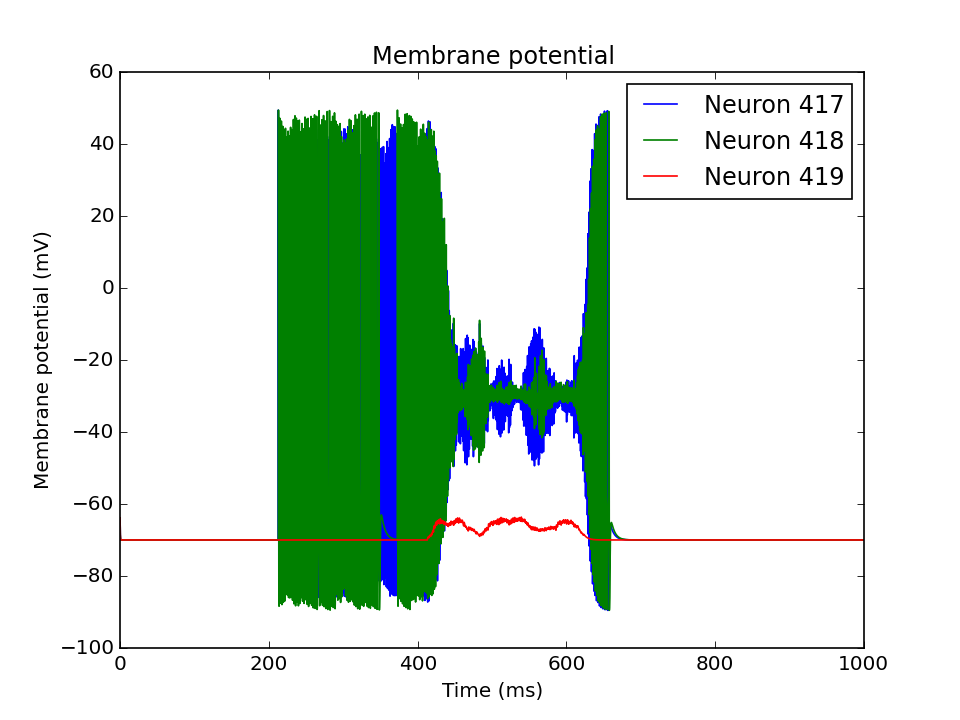
\includegraphics[width=0.5\linewidth]{bad_amygdala}
	\caption{Устранённая мутация потенциала мембраны перестимулированного нейрона в нейронах миндалевидного тела (зелёный, синий).}
	\label{fig:bad_amygdala}
\end{figure}

Вопрос о балансировании влияния серотонина на дофамин становится определяющим для реализации таких вычислительных эмоций, как радость и интерес. По модели Левхейма, эти эмоции возникают при высоких уровнях серотонина и дофамина, однако ингибирующее действие серотонина на дофамин почти исключает возможность их одновременной активности. Была проведена работа по настройке весов серотониновых и дофаминовых связей для их сбалансированного действия.


Ответом на вопрос о вычислительной машине с характеристиками, достаточными для проведения симуляции на полумиллионе нейронов с более миллионом связей между ними, стал IBM кластер из компьютеров-хостов, предоставленный поддержкой Казанского федерального университета. Cимуляция длилась 5 суток.